The marine ecosystem model used in this study is the Apex Predators Ecosystem Model (Apecosm, \citealt{mauryModelingEnvironmentalEffects2007, mauryOverviewAPECOSMSpatialized2010}), which simulates the transfer of energy in marine ecosystems in a 5 dimensional space (space, time, community and size). The biological processes include size-based opportunistic trophic interactions, competition for food, allocation of energy between growth and reproduction, somatic and maturity maintenance, predatory and starvation mortality (see \citealt{mauryModelingEnvironmentalEffects2007} for a detailed description of the model). The physiological bases of the model are derived from the Dynamic Energy Budget theory (DEB, \citealt{kooijmanDynamicEnergyMass2000}). All the physiological rates are temperature-dependent. In addition to biological processes, energy density is also subjected to both passive and active advection/diffusion, following \cite{faugerasAdvectiondiffusionreactionSizestructuredFish2005}

Changes of fish biomass induced by growth is given by:

\begin{equation}
\partial_t \varepsilon = - \partial_w(\gamma \varepsilon) + \frac{\gamma}{w}\varepsilon
\label{eq:growth}
\end{equation}

where $\varepsilon$  is the fish biomass density, $w$ the weight and $\gamma$ is the growth rate. Changes driven by predation mortality are given byL:

\begin{equation}
\partial_t \varepsilon = - M \varepsilon
\label{eq:pred}
\end{equation}

where $M$ is the predation mortality rate, computed using equation 12 of \cite{mauryIndividualsPopulationsCommunities2013}. 

Finally, changes in fish biomass induced by fish movements are given by:

\begin{equation}
\partial_t \varepsilon = -\overrightarrow{\nabla}.(\overrightarrow{V} \varepsilon) + \overrightarrow{\nabla} . (D \overrightarrow{\nabla} \varepsilon)
\label{eq:move}
\end{equation}

with the first term being the contribution of advection and the second term being the contribution of diffusion, $V$ the velocity (which is the combination of active speed and ocean currents) and $D$ the diffusivity coefficient (which is the combination of an active, i.e. foraging, diffusion term and a passive diffusion coefficient).

In order to ensure that the size-spectrum is fully unfolded, the model has been integrated three times. First, the model has been initialized from rest and run from 1958 to 2018, using the outputs of the NEMO-PISCES simulation. Then, the end of this first spin-up phase has been used to run another cycle, which was in turn used to run the simulation presented in the given study.

In order to assess the mechanisms of fish biomass response to ENSO variability, biomass changes induced by growth, predation, advection and diffusion are stored for the entire simulation. Therefore, the biomass for a given size class, at a given location and for a specific time can be reconstructed by using the following equation:

\begin{equation}
\varepsilon(x,y,T) = \varepsilon(x,y,T=0) + \int_{t=0}^{T} \left[ 
T_{pred}(x, y,t) + 
T_{growth}(x, y,t) + 
T_{adv}(x, y,t) + 
T_{diff}(x, y,t) 
\right] dt 
\label{eq:rec_oope}
\end{equation}

with $\varepsilon(x,y,T=0)$ the fish biomass at the beginning of the simulation and $T_{pred}$, $T_{growth}$, $T_{adv}$ and $T_{diff}$ the respective biomass increments due to predation, growth, advection and diffusion, given by equations \ref{eq:pred}, \ref{eq:growth} and \ref{eq:move}, respectively.

In the present work, three generic communities are simulated: one epipelagic community, one migrant community and one mesopelagic community. The epilagic community remains close to the surface its vertical distribution is influenced by temperature and oxygen, while light only influences their functional response. The migrants are only influenced by light, which modifies their vertical habitat and their functional response: during daytime, they remain at depth, while moving at the surface at night for feeding. Mesopolagics, on the other hand, remain at depth during both night and day, their vertical distribution being only impacted by the light. 
%Epilagic feed on other epilagic fish only during night daytime. Migrants feed on other migrants and epipelagics, only during night-time. While mesopelagics feed on migrant and mesopelagic during daytime, and only on other mesopelagic during night-time.

Since the epipelagic are close to the surface (around $50m$), they are likely to be more impacted by ENSO variability, as suggested by \cite{lemezoNaturalVariabilityMarine2016}. Therefore, in the following, we will mainly focus on this specific community. Furthermore, for the sake of simplicity, we will detail the results for three size classes: 3cm, representing small fishes, 20cm, representing intermediate sizes, and 90 cm, representing large individuals. The latter are representative of the sizes of tuna target species within the region (\warn{REF}). \\

Before analysing the mechanisms of fish biomass response to El Nino variability, simulated biomass is compared with observation-based estimates. Simulated fish biomass and catches have been integrated between 10N and 10S. Figure \ref{fig:apecosm_validation} shows the Hovmoller diagram of the observed catches and fish biomass (log-scale) for the 1900-2018 period.
First, one can notice that the barycenter of catches moves eastward over time. This shift can be explained by the increased power of fishing fleets, which allow them to move further east (\warn{REF}). Although the agreement between the observed and simulated barycenters is not clear, some observed patterns are well captured by the model. For instance, the easternmost $7.00$ simulated contour seems to closely follow the eastward extension of catches that occur between 2002 and 2018 (in 2010-01, 2012-01 and 2016-01 for instance). Therefore, we can assume that Apecosm realistically simulates fish variability and can be used to infer the underlying mechanisms.

\begin{figure}
	\centering
	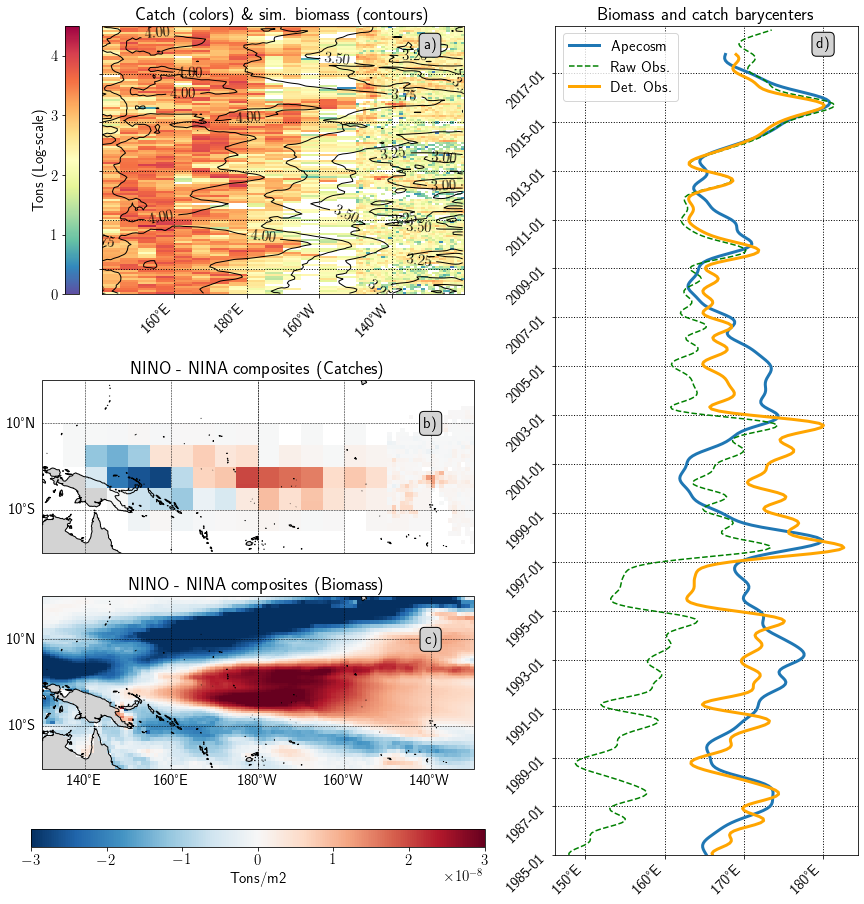
\includegraphics[scale=0.5]{figs/plot_validation_apecosm.png}
	\caption{Hovmoller diagram of observed catches (colors) and simulated fish biomass (contours) integrated between 10N and 10S (log-scale). The black and blue lines show the longitude of the barycenters of fish biomass and catches, respectively.}
	\label{fig:apecosm_validation}
\end{figure}
